\chapter{Question 1}
\label{intro}

\textbf{Demonstrate that you know how to use ``curl'' well enough to correctly POST data to a form. Show that the HTML response that is returned is ``correct''.  That is, the server should take the arguments you POSTed and build a response accordingly.  Save the HTML response to a file and then view that file in a browser and take a screen shot.}\\

To POST data to a form using cURL, I did the following:
\begin{itemize}
\item I created a form using PHP with name as an input element and a submit button.

\item When we open this PHP form in the browser and type any name, it displays a response saying ``Welcome followed by the text''.

\item By using the following cURL command we can POST data to the form which is received by the server and generates a response with the same message that we see on the browser. By using -o followed by parameter, I am outputting the HTML response to a file.
\end{itemize}
\begin{verbatim}
 curl -d name=Srividya ``www.cs.odu.edu/~smajeti/postForm.php'' 
 -o output.html
\end{verbatim}


\newpage

\lstinputlisting[language=PHP,caption=``PHP script'',frame=single,breaklines=true,captionpos=b,numbers=left,showspaces=false,showstringspaces=false,basicstyle=\footnotesize]{src/postForm.php}

\begin{figure}[h!]
\begin{center}


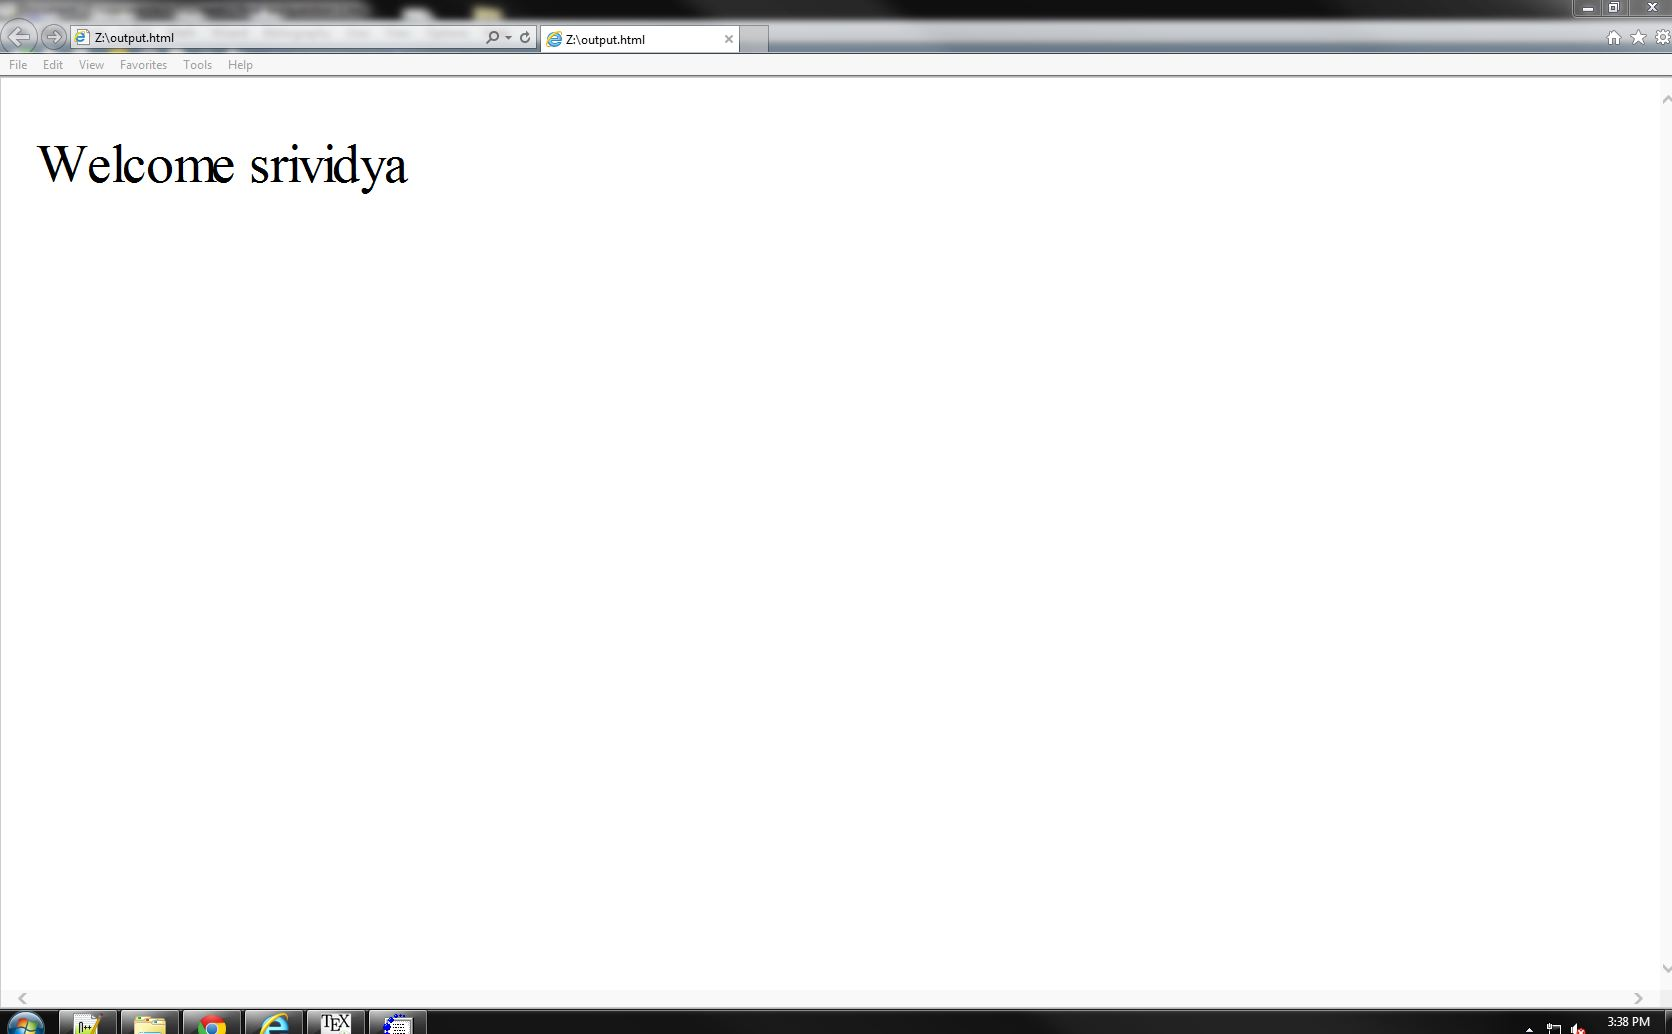
\includegraphics[scale=0.30, keepaspectratio=true]{figures/q1screenshot.JPG}
\caption{HTML response saved into a file and viewed in browser.}
\label{mcpon_navy_mil}
\end{center}
\end{figure}
